\section{Results}\label{sec:results}

The evaluation of our system is conditioned by the fact that there is no ground truth available to assess its quality. To evaluate our system, we decided to present three bills as case studies and to show the insight and short-comings of our method in the generation of Policy Networks. For each of these bills, we present a brief description so that the reader understands their context and show some of the most relevant PNs that we generated. 

\subsection{BCN-World}\label{subsec:bcn_world}

BCN-World is a tourist and entertainment project which was announced in 2012. The project included several hotels, casinos and gambling houses, theme and water parks, golf courses, a beach club, theaters, convention centers, shopping malls, restaurants, among others. BCN-World was planned to be built in Tarragona, a province of Catalonia which is located to the south of Barcelona. \\

The project was largely promoted by Veremonte, a british based investment group, and Convergencia i Uni\`o (CiU), a right-wing party currently governing in Catalonia. Veremonte coordinated the efforts of several other investment groups, including La Caixa - a Catalan bank -; Melco and Caesars Entertainment - two Asian and American based leisure and gambling corporations -; Hard Rock; Value Retail - a luxury outlet shopping company- and Melia Hotels. \\  

Because of the enormous size of the project, its implementation required the modification of the law regulating every aspect of a Touristic Complex. The new bill, written in 2014, took into account all the negotiations between the investors and the Catalan Parliament. For instance, given the significant involvement of gambling companies in the project, lowering the gambling industry taxes from $55\%$ to 10\% was a necessary pre-condition for the execution of the project. \\

The negotiations between the investors and the Catalan government were conditioned by the fact that the ruling party, CiU, does not have a majority and has required the support of a left wing party called Esquerra Republicana de Catalunya (ERC). ERC was opposed from the very start to the bill. Because of this, CiU had to look for the support of other political parties, and found an ally in the Partit dels Socialistes del Catalunya (PSC, the Socialist Party of Catalunya). Despite initially being against the project, the PSC changed its position because it rules in the cities located near BCN-World and its mayors were interested in the execution of the project as a means to create employment in their districts. After intense negotiations including the mayors and senior politicians of the PSC, CiU got the necessary votes to approve the new law regulating Touristic Complexes.

\subsubsection{Organization-Organization PN}\label{subsec:bcn_world-company-company}

Figure \ref{fig:00062014-organizations} shows the PN relating the main organizations concerned by the BCN-World bill. Due to space constraints, we show only the giant component of this network. The nodes of the graph are coloured according to the communities detected by performing modularity clustering. The size of the nodes and the font of the names are proportional to their Pagerank centrality. Pagerank is a metric widely used in Social Network Analysis to assess the importance of a node. The Pagerank algorithm assigns to each node a value that is computed based on the number and quality of its links to other nodes. The idea is that a node is as important as the number of links it receives from other important nodes.\\

There are several insights that can be derived from the Organization PN. To start with, three main communities are detected. The first community, in dark red and in the upper left part of the graph, is mostly composed of political parties and other NGO which are linked to these. ERC, Ciu, CUP, ICV-EUIA, PP, PPC and Ciutadans are political parties, while ACENCAS (Associaci\'o Catalana d'Addiccions Socials) is the Catalan Asociation of Social Addictions, Camara Catalana (Cambra Catalana) is the Catalan Chamber of Commerce, Parlament is the Parliament, Govern refers to the Government and Tripartito and Sociedad Centre Medics Selva Maresme are noisy entities which are not related to the bill. All of the political parties are related among themselves and with the Government, the Parliament and the Chamber of Commerce. ACENCAS, an organization which was opposed to the bill, is shown to be linked with CUP, another left wing party which was very strongly against BCN-World. \\

The second community, shown in dark pink and in the lower right section, is mostly constituted by the companies interested in investing in BCN-World. Note that none of these companies are related to the political organizations except for Veremonte. This is due to the fact that Veremonte, as we previously established, was the intermediary between the investors and the government. Its bridging role is clearly shown in this PN. \\

The last community, in light pink and the lower left part, is composed mostly of institutions from Tarragona, the province where BCN-World was set to be built. This includes the local government (Diputaci\'on de Tarragona, in catalan Diputaci\'o de Tarragona), the local chamber of commerce (Camara de Comercio de Tarragona, in catalan Cambra de Comer\c{c} de Tarragona), the Confederation of Tarragonian Business (CEPTA), the Port of Tarragona and Universitat Rovira i Virgili (an university based in Tarragona). There are other organizations that are not related to Tarragona, including the Spanish Association of Accountants, La Caixa (a Catalan bank) and Pimec which stands for Small and Median Businesses. Note however the important role of Diputacion de Tarragona as determined by its pagerank value. This confirms its role as a broker between the Catalan Government and Veremonte.

\begin{figure}[H]
    \centering
    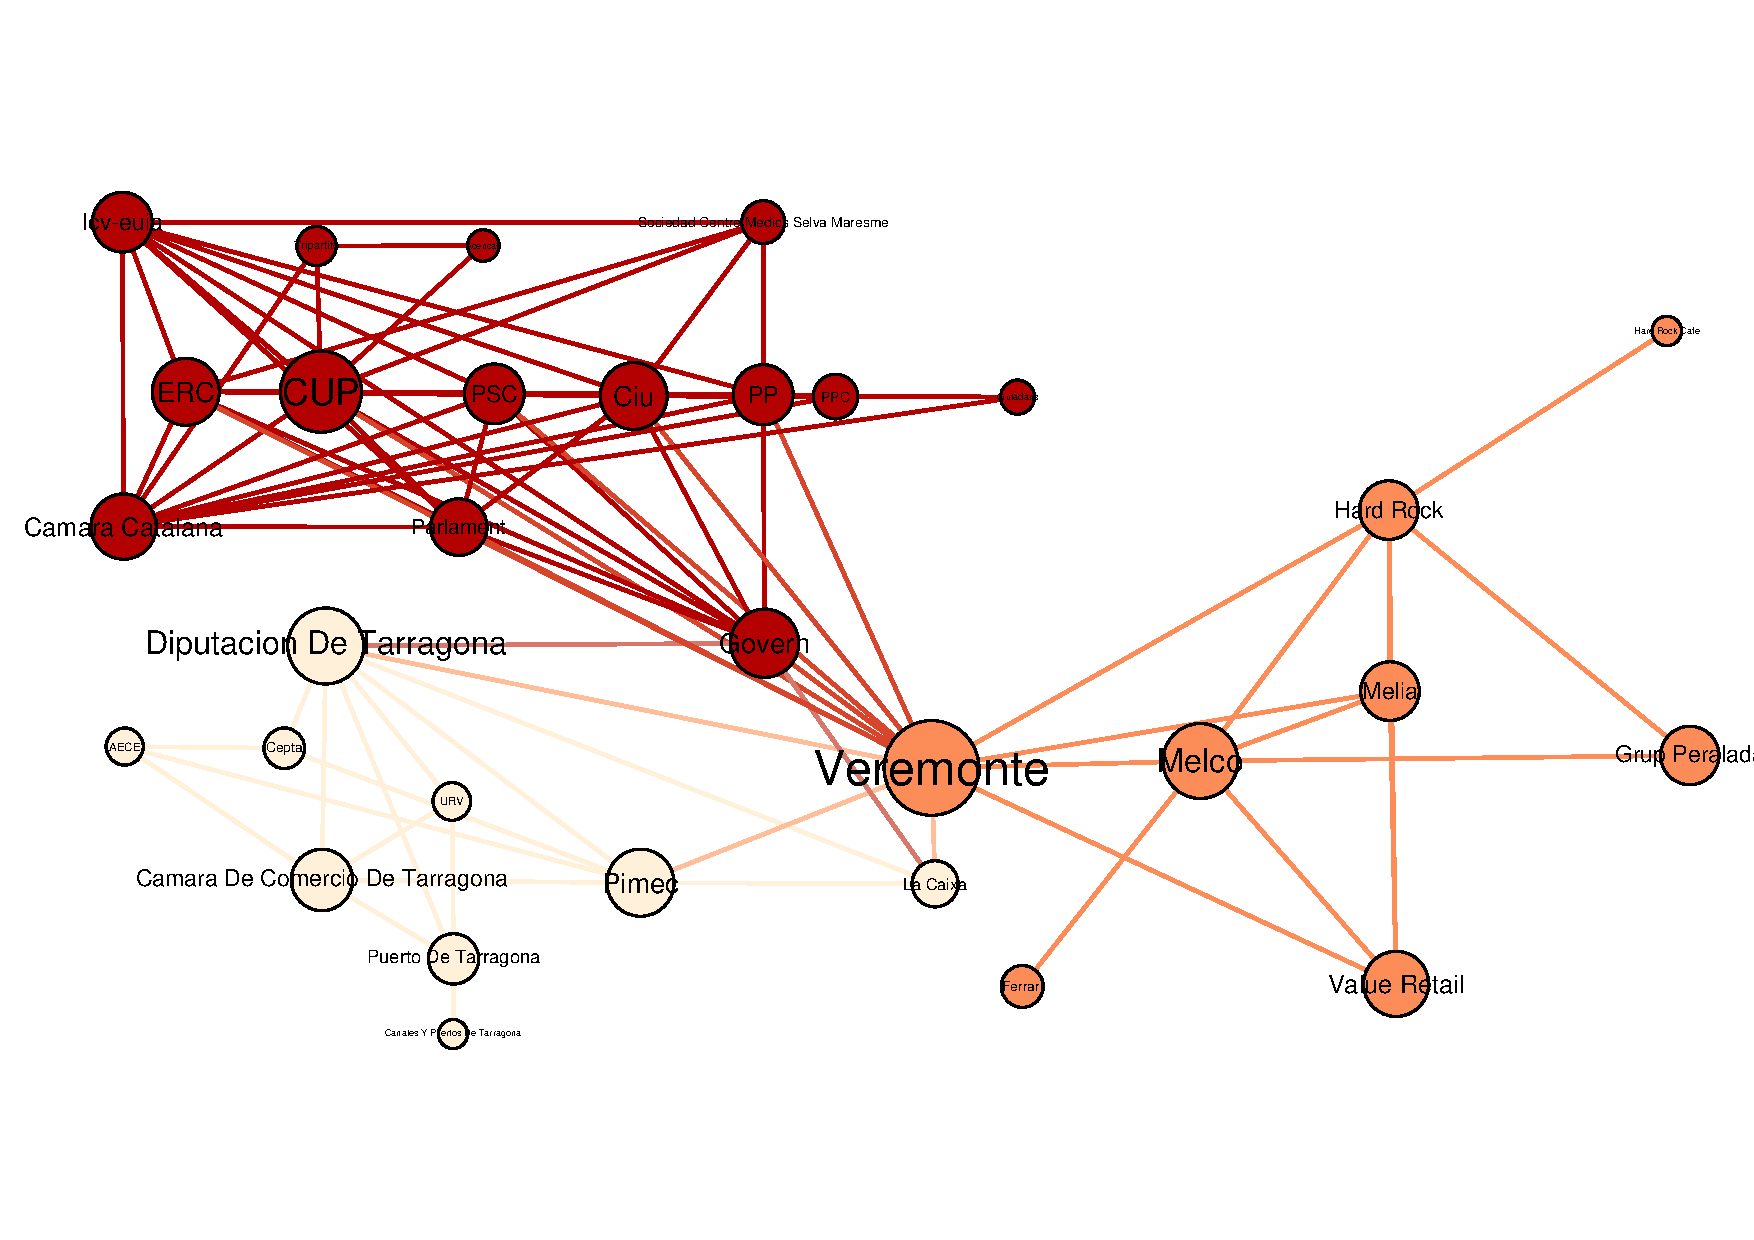
\includegraphics[width=0.9\textwidth]{figs/00062014-organizations}
    \caption{Organizations PN of the BCN-World Bill.}
    \label{fig:00062014-organizations}
\end{figure}


\subsubsection{Person-Organization PN}\label{subsec:bcn_world-person-organization}

Figure \ref{fig:00062014-organizations} shows the PN relating the relationships between the most important persons and organizations related to BCN-World. This graph was constructed by considering all possible relationships between persons and organizations, selecting the most influential persons and organizations as measured by their pagerank and filtering out every node that is not relevant or directly connected to a relevant node. Once more, we show only the giant component due to space constraints.\\

\begin{figure}[H]
    \centering
    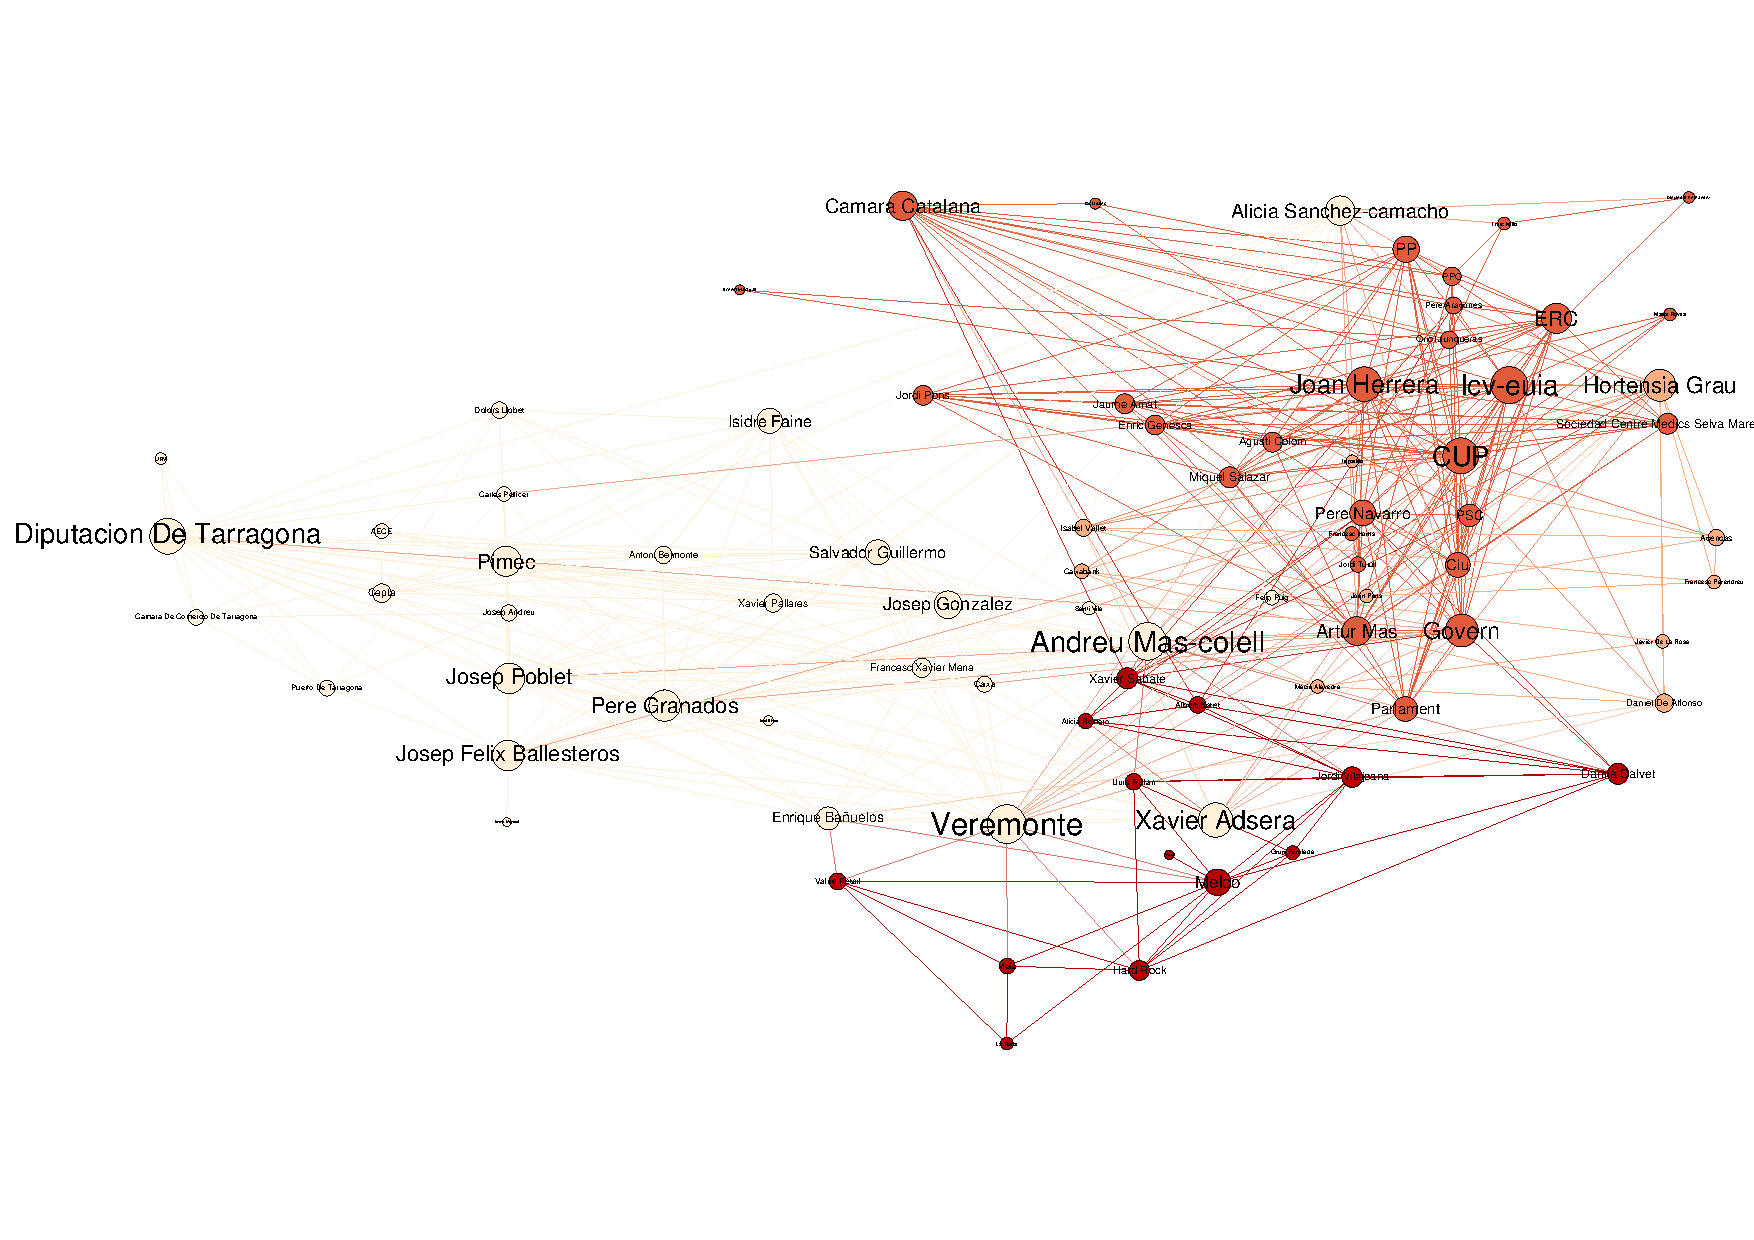
\includegraphics[width=0.9\textwidth]{figs/00062014-person_organizations}
    \caption{Person-Organization PN of the BCN-World Bill.}
    \label{fig:00062014-organizations}
\end{figure}


This graph is bigger in number of nodes but is similar to the Organization-Organization PN. To start with, it features three communities which are related to the communities previously found: a community formed by investors (in the lower right corner), a community of politicians and their political parties (in the upper right corner) and a community of organizations and people related to Tarragona (in the left side). \\
Note that the most relevant actors from the Organization-Organization PN retain their importance: Veremonte, Diputaci\'o de Tarragona, CUP and the Government are highly central. Cambra Catalana (The Catalan Chamber of Commerce) is now slightly more important, as it has many connections with politicians. \\

When it comes to analyzing the role of persons, there are many interesting insights to be gained. First, the most relevant people are Andreu Mas-Colell, the Advisor of Economy and Knowledge of the Catalan Government, and Xavier Adsera, a senior advisor to Veremonte and the president of the BCN-World group. Other relevant entities include Josep Felix Ballesteros, Pere Granados and Josep Poblet, three PSC and CiU mayors of the main towns in Tarragona; Joan Herrera and Hortensia Grau the spokesmen of ICV-EUIA, a party against the project; Artur Mas, the president of the Catalan Government;  Alicia S\'anchez-Camacho, spokeswoman of PP, the ruling party in Spain and Isidre Faine and Enrique Ba\~nuelos, presidents of La Caixa and Veremonte. \\

Something which is particularly interesting is how there intermediary role of Veremonte is reinforced in this PN, showing links with most of the nodes in the other two communities and being also connected to them through Xavier Adsera. By inspecting the news articles, we realize that Adsera was the main negotiator for Veremonte and participated in several key meetings, for instance with Ballesteros, Granados and Poblet, to convince the PSC to vote in favor of the law. \\

An Organization-Person-Person-Organization graph pattern like this might be particularly interesting for detecting lobbying relationships. We find for instance that Veremonte is directly conected to the Catalan Government; these are two organizations that are in turn related to Adsera and Artur Mas who are brokers in charge of connecting their respective organizations. \\

Besides from these interesting insights, this graph also shows some shortcomings of our method. First, there is a giant community made of politicians which does not seem to exhibit any kind of internal sub-structure. Almost all of the politicians of the Parliament are connected with every other politician, instead of, for instance, showing only connections among politicians of the same party. \\

A second shortcoming of this graph is that it fails to detect some relationships which are very important. For instance none of the previously mentioned mayors are related to their political party, something which is particularly important to establish their role as negotiators. This might be because they are mostly referred in the news as mayors of important cities of Tarragona (note how they are strongly linked to most of the institutions of the Tarragona community) instead of being related to their political parties. 


\subsection{Law of Popular Non-referendary Consults}\label{subsec:lpnc}

The Law of Popular Non-referendary Consults (hereinafter LPNC) is a law which was approved in September 2014 to allow the Catalan Government to call for non binding electoral consults to catalan citizens. This law was particularly controversial as it was approved with the main objective of making a consult regarding Catalonia'secession from Spain. Shortly after its approval, Artur Mas, president of the Catalan Government, called for such a consultation to take place on November 9th. The Spanish Government immediately declared its unconstitutionality, which the Supreme Court of Spain availed. \\

The LPNC is particularly interesting because although its a law regulating any type of consultation on public affairs, its controversy lies on its use for the November 9th election. The affected parties are consequently mainly politicians and organizations which are in favor or against Catalan independence.\\

\subsection{Organization PN}\label{subsec:lpnc-organization-organization}

Figure \ref{fig:00062014-organizations} shows the Organization PN for the LPNC. As previously, colors identify communities and font and node size identify importance as measured by the Pagerank of the node. We show only the giant component of the graph.\\


The first relevant observation is that the entities shown in this graph are mostly political parties and NGOs related to the independence of Catalonia. Modularity Clustering yields three communities, shown in the upper left, upper right and bottom sections of the graph. The two communities in the the upper right section are made on the one hand by parties of Spain, Catalonia and other regions of Spain which have independentist claims and, on the other hand, institutions that were involved in determining its constitutionality: the Spanish Senate and House of Representatives (\emph{Senado} and \emph{Congreso}), the Catalan Parliament(\emph{Parlament}) and the Constitutional Court of Spain (\emph{Tribunal Constitucional}). The single community in the bottom of the graph mostly shows pro-independence groups: \emph{Barcelona Decideix}, \emph{Reagrupament}, \emph{Solidaritat} and \emph{Moviment Arenyenc}. \\


\begin{figure}[H]
    \centering
    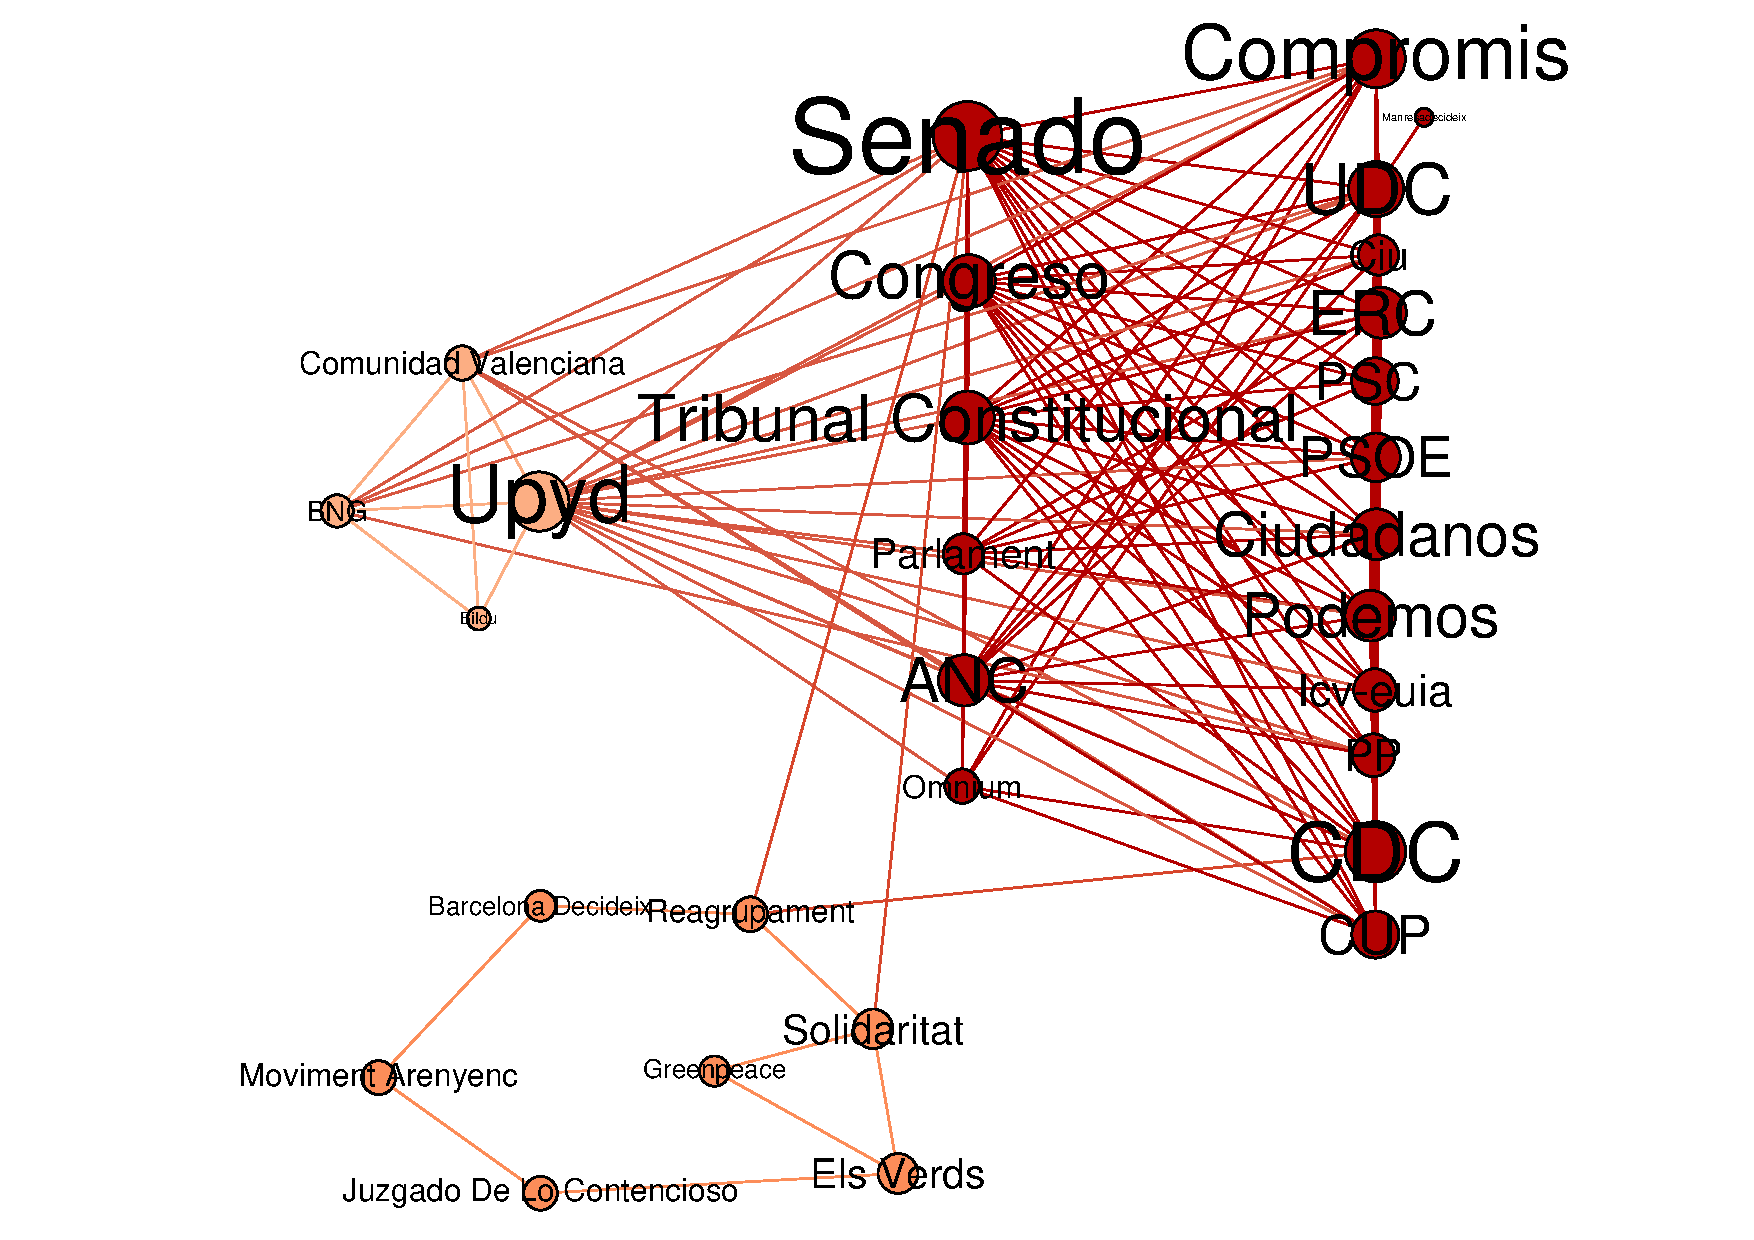
\includegraphics[width=0.9\textwidth]{figs/00102014-organizations}
    \caption{Organization PN for the LPNC bill}
    \label{fig:00102014-organizations}
\end{figure}


Broadly speaking, these communities correctly identify the two types of organizations that are involved with the law, with some exceptions: \emph{ANC} (Assemblea Nacional Catalana, in English National Catalan Assembly) and \emph{Omnium} are NGOs which rather than being connected with the rest of the NGOs are connected with other political parties. This might seem counter-intuitive at first, but if may be because they work more with political parties than with the rest of NGOs. Similarly \emph{Juzgado de lo Contencioso} (Litigation Court) would intuitevely be related with the rest of the political institutions. Finally, note how \emph{Greenpeace} and \emph{Els Verds}, despite not being related, are present in the graph. These might be due to the fact they are too Non-Governmental Organizations, devoted though to environmentalist causes. 

When it comes to assessing the importance of organizations, we find that almost all the political parties, with the exceptions of parties from other regions of Spain, are equally relevant as measured by Pagerank. Also note the importance of the Spanish Senate and Congress, the Catalan Parliament and the Constitutional Court. Among the pro-Independence NGOs, \emph{ANC} is the most preeminent.

\subsection{Person PN}\label{subsec:lpnc-person-organization}

Figure \ref{fig:00102014-persons} shows the Person PN for the LPNC. When analyzing the community structure of the PN, we see that there are seven communities, identified with different colours. In the case of this PN its hard to make sense of the clusters of people identified by modularity clustering. Politicians of different parties and of different regions or instutions, are spread around the graph. \\

On the other hand, looking at individual, widely known politicians, it is possible to make sense of the relations we see. For instance, Mariano Rajoy, the prime minister of Spain, is connected to senior members of PP, his political party, and of other relevant parties. Similarly, senior pro-independence politicians like Artur Mas, Oriol Junqueras, Josep Antoni Duran tend to be connected together. \\

\begin{figure}[H]
    \centering
    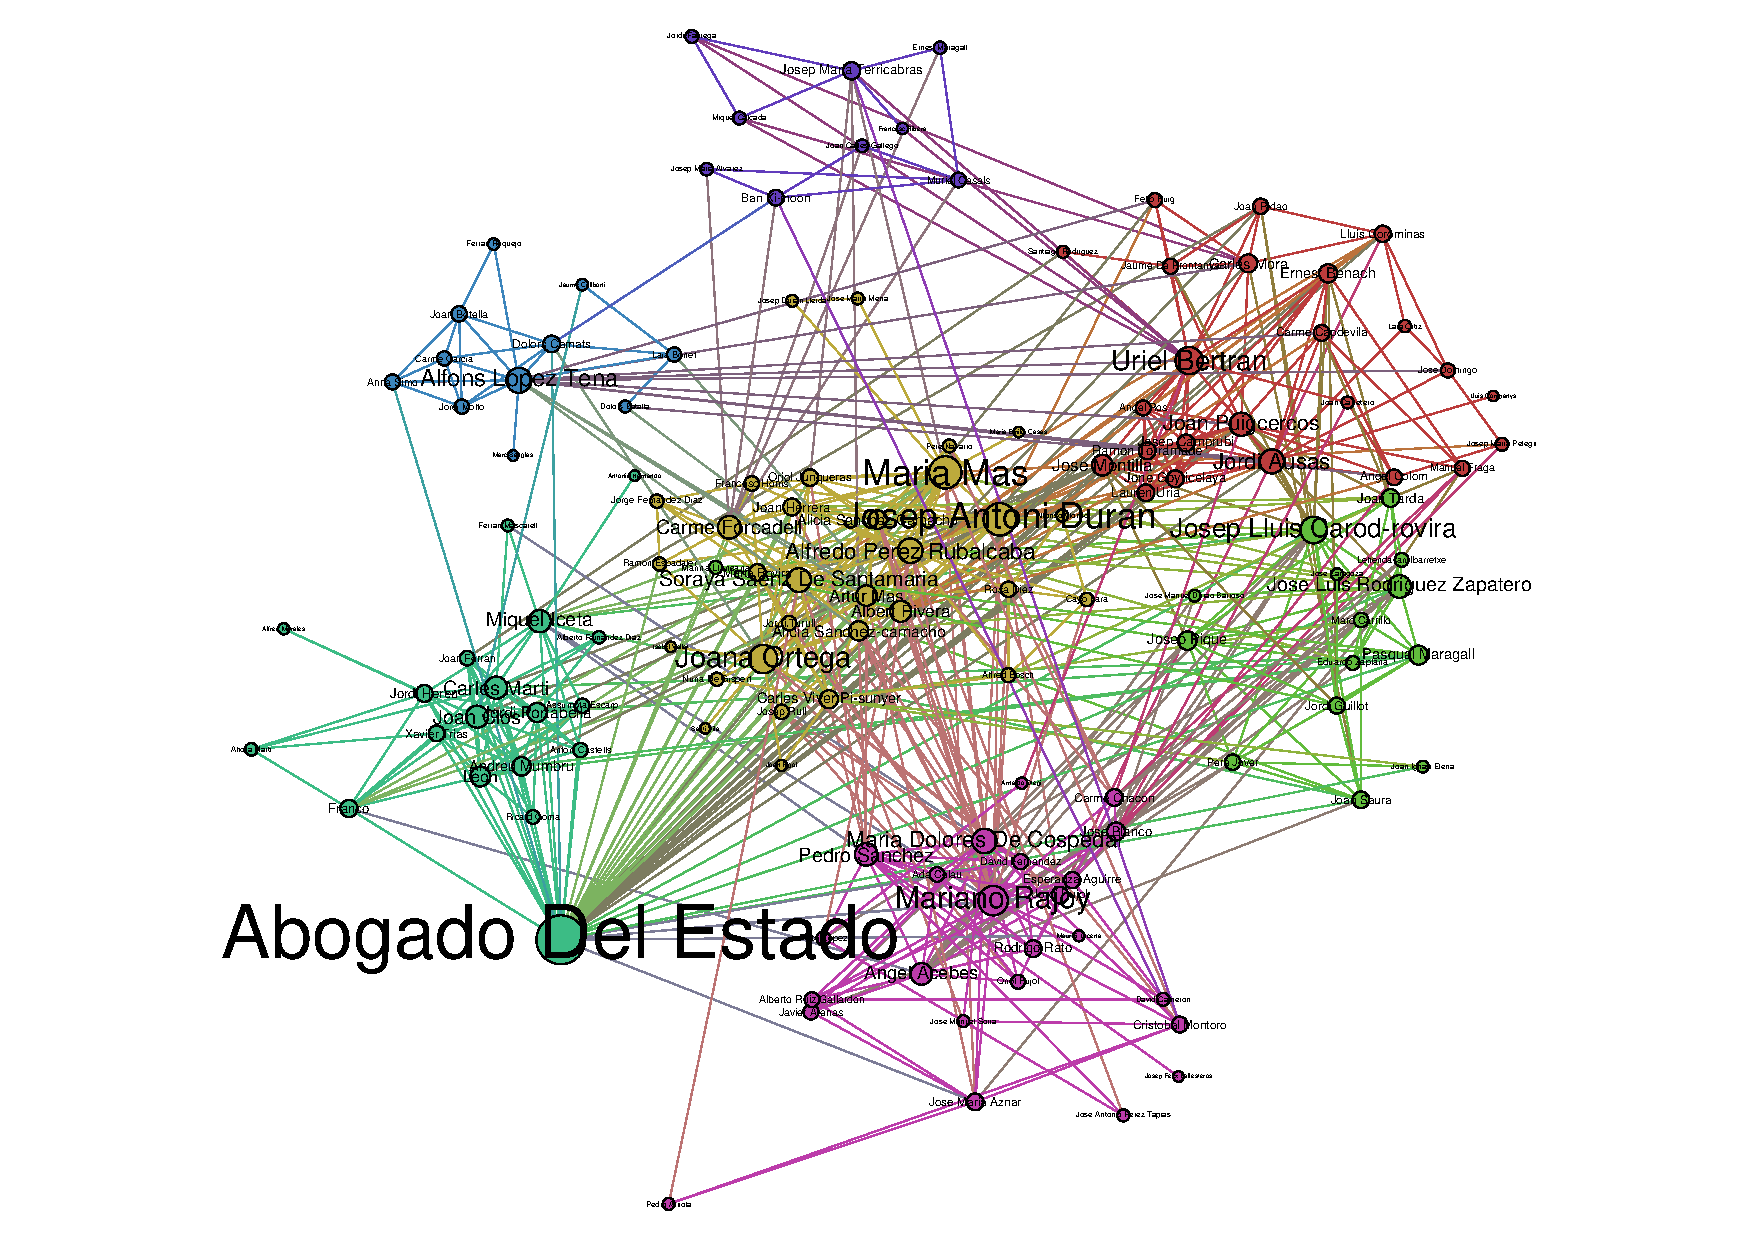
\includegraphics[width=1\textwidth,scale=1.3]{figs/00102014-persons}
    \caption{Person PN for the LPNC bill}
    \label{fig:00102014-persons}
\end{figure}



